\def\year{2017}\relax
%File: formatting-instruction.tex
\documentclass[letterpaper]{article} %DO NOT CHANGE THIS
\usepackage{aaai17}  %Required
\usepackage{times}  %Required
\usepackage{helvet}  %Required
\usepackage{courier}  %Required
\usepackage{url}  %Required
\usepackage{graphicx}  %Required
\usepackage[ruled,vlined]{algorithm2e}
\usepackage{comment}
\usepackage{amssymb}
\usepackage{subcaption}
\frenchspacing  %Required
\setlength{\pdfpagewidth}{8.5in}  %Required
\setlength{\pdfpageheight}{11in}  %Required
%PDF Info Is Required:
  \pdfinfo{
/Title (Supervised Reinforcement Learning with Partial States: a Teaching Method for Action Selection for HRI)
/Author (Emmanuel Senft)}
\setcounter{secnumdepth}{0}  
 \begin{document}
% The file aaai.sty is the style file for AAAI Press 
% proceedings, working notes, and technical reports.
%
\title{Supervised Reinforcement Learning with Partial States: \\
 a Teaching Method for Action Selection for HRI}

\author{Emmanuel Senft \\
CRNS \\
Plymouth University \\
United Kingdom\\
\And S\'{e}verin Lemaignan\\
CRNS \\
Plymouth University \\
United Kingdom\\
\And Paul Baxter\\
L-CAS\\
University of Lincoln\\
United Kingdom\\
 \And Tony Belpaeme\\
 CRNS\\ Plymouth University (UK) \\ iMinds \\ Ghent University (Be)}

\maketitle
\begin{abstract}
%As robots will integrate human society, they will have to satify humans'
%expectations. However at the design time, it seems hardly possible to
%know in advance exactly all the behaviours expected from the robot. As such to
%be accepted in human society robots have to learn how to interact with humans.
    Learning social interactions is a complex task that robots will have to
    master before being accepted in society. However, as no simulator of human
    interactions sufficiently
    precise exists today, the learning have to be made online and in the real
    world. Actions executed by the robot have impact on humans, and as such
    have to be carefully selected, making the reliance on random exploration not
    applicable. Additionally, no clear reward function exists for
    social interactions. This implies that classical approaches such as
    Reinforcement Learning cannot be directly applied. As such we argue that
    robots will highly profit from human expertise and guidance to learn social
    interactions. And as the quantity of input a human can provide is limited,
    new methods have to be designed to use more efficiently human inputs. We
    combine the Supervised Progressively Autonomous Robot Competencies (SPARC)
    allowing a safer online learning with Reinforcement Learning based on
    partial states rather than full states to accelerate the learning by
    collecting and using more information from the human teacher.
\end{abstract}
%===============================================================================

\section{Introduction}

Human-Robot Interaction (HRI) aims at having humans and robot living together
in the society, interacting socially in many different environments and
contexts. Robot are expected to behave appropriately regardless of the domain
of interaction. However, not all behaviours can be known in advance and be
implemented in the robot before its deployment in the real world. Similarly to
 humans, robots need
to be able to learn new tasks, new actions policies, new social norms and how
to make sense of the world surrounding them.

For a robot, interacting in the real world requires to combine inputs
 from many sensors to create a space composed of large number dimensions and
select actions appropriated to the current space. However,
 parts of the state can be irrelevant to the current goal and are not required
 to be taken into account to select the current action. A successful action
 policy maps these features to the relevant actions.

These relevant features in the space can be encoded in the representation of
the space the robot uses for action selection or be learnt. Recent successes in Deep
Learning~\cite{lecun2015deep} have shown that complex features can be extracted
by neural networks assuming that enough datapoints are available. 

In previous work~\cite{senft2015sparc,senft2017supervised}, we introduced the
Supervised Progressively Autonomous Robot Competencies (SPARC), as a way to
teach a robot an action policy while interacting based on a supervisor
correcting actions about to be executed by the robot. In this paper, we propose
to extend this approach to allow the supervisor to highlight features in the
environment associated to the selected action. During the action selection
phase, the robot can compare these features, defined as partial states, with the
current state to select an action based on which previously identify
features are currently in the environment.

\begin{comment}
This approach in especially relevant for HRI as gathering datapoints has to be
performed in the real world and interacting with humans forces a robot to have
an appropriate action policy at anytime of the interaction. even in the early
phase when the robot has no information about the way its environment react to
its actions. 

When interacting in the real world, humans face huge spaces of almost unlimited
dimensions, and despite this complexity, humans, and especially children are able
to learn quickly, often from only a few demonstrations or examples. One of the
 reason could be that they are able to take the most out of every datapoint available to them. 
 On the other
hand, recent impressive advances in Machine Learning such as Deep Learning~\cite{lecun2015deep}
have been made possible by the availability of huge dataset covering millions
of labeled examples or dozens of hours of recording. These progress have
targetting either perception, where labeled datapoints can be available or
action selection in virtual environments where the impact of actions is
limited.

However, these large labelled dataset or virtul worlds do not exist for
social interaction. To learn how to interact with humans, robots have to
experiment in the real world facing the actual reactions from their actions. As
such they
have to learn quickly while consistently exhibiting a acceptable behaviours.
One way of ensuring this correct  behaviours is to rely on a human to supervise
the robot during the early phase of learning, and this human can also provide
inputs to boostrap the learning, achieving a faster learning. This paper present
a novel method based on human supervision, feature highlighting and partial
state reinforcement learning to achieve this fast and safe learning.
\end{comment}
%===============================================================================

\section{Background}
\subsection{Reinforcement Learning}

The main framework for an agent to learn how to interact in an environment while
interacting is Reinforcement 
Learning (RL)~\cite{kober2013reinforcement,sutton1998reinforcement}. In RL, an
agent is interacting in an environment
providing numerical reward in reaction to the agent's actions and
the agent learns an action policy to maximise the expected cummulative discounted
reward obtained by the agent.

Classic approaches in RL generally rely on exploring virtual environments where the agent
tries to maximise the reward. In many cases where RL achieves success, the agent
had access to a virtual environment where the only real cost of exploring was 
time and energy, and the agent can interact as long as needed to gather
enough information on the environment to find a correct action policy. When
these conditions are reunited, RL can achieve impressive results, as shown by
the victory of a computer in Backgammon back in the
90s~\cite{tesauro1995temporal} or more recently the success achieved in playing
Atari games based only on the image and the game rewards~\cite{mnih2015human}.

\subsection{Human impact on Reinforcement Learning}

Initial knowledge is often a crucial step to allow an algorithm to learn an
efficient action policy. This knowledge, originating from human expertise, can
be exploited in many ways. 

\subsubsection{Design decisions:}
Initial knowledge has to be use in the designing of the algorithm, the
representation of the state and actions spaces and the rewrd funtion. For
example, only carefully crafted features allowed
Tesauro to improve its algorithm for Backgammon from a intermediate-level player
to super-human level~\cite{tesauro1995temporal}. Similarly, the design of
complex neural networks for state generalisation, the representation of actions
as motor primitive rather than raw motor angles or adding additional
informations in the reward function have important impacts on the ability of
the robot to reach a successful policy.

\subsubsection{Demonstrations:}
Initial knowledge can be provided to the agent learning through demonstrations.
These demonstrations can be used to create an initial policy sufficiently
efficient to start interacting in the environment and gather information to
improve over time. This initial policy, required to receive meaningful feedback
from the environment can be impossible to reach by relying only on random
exploration and feedback from the environment. For example the game of Go in its larger board
size contains more than $10^{210}$ states, so exhaustive search is not possible.
Authors of \cite{silver2016mastering} started with
supervised learning from go master's games to learn a decent policy and then
used deep learning, self play and tree search to achieve super-human
capabilities and beating humans best players.

These demonstrations can also be used to learn a reward function. With Inverse
Reinforcement Learning, the agent is not provided with a reward function, but
derives it from a set of expert demonstrations. The agent can then explore
around the demonstrated policy to find how to optimise the reward function. With
this approach, Abbeel and Ng achieved better than human control for a robotic
helicopter~\cite{abbeel2004apprenticeship}.

\subsubsection{Guiding the learning:}

In some cases, the state space is simply too big to rely only on random exploration to
reach a successful action policy.Rather than solely providing initial knowledge
to the agents, humans can also guide the agent throughout the learning in a more
human-like teaching manner. 

A first approach consists in sequencing tasks the robot will face. 
This approach, known as "scaffolding" \cite{saunders2006teaching}, progressively
increase the difficulty and complexity of the task or the environment as the
robot is learning policies to achieve complex task not directly learnable in the final
environment.

A second approach is "shaping". For example, the TAMER framework
\cite{knox2009interactively}, allows to teach an agent an action policy in an
environment providing no rewards using a human observer to supply rewards to the
agent. With this approach the teacher can adapt the
rewards to the current policy and performance of the agent, for example starting to reward
positively suboptimal behaviours but which still improve the current policy and
later, as the agent improve its behaviour reward these same suboptimal behaviour
negatively and only the optimal ones positively.

Another approach to guide the the learning is to bias the action selection.
In~\cite{thomaz2008teachable}, the authors propose to use a human supervisor to
supply  an agent both rewards and potential guidance or advise indicating where
the agent should pay attention, or what it should do next. And they show that
giving the power to the supervisor to bias the action selection can improve the
learning, making it faster, safer.

In \cite{senft2015sparc}, we introduced the Supervised Progressively
Autonomous Robot Competencies (SPARC). SPARC relies on the presence of a
supervisor teaching a robot how to interact in an environment. This teacher
knowns which actions the robot is about to execute and can cancel an action or
select another to be executed. Based on the supervisor's decisions, the robot
learns which actions are desired and can refine its policy over time reducing
the need for the teacher to correct or select an action.

SPARC gives control on the robot actions to an expert, who can guide the
exploration in the desired part of the environment and this ensures the robot's
behaviour is consistently appropriate. As the exploration is
guided, and all the actions are useful, the learning can be faster than
autonomous learning or feedback based learning as illustrated in Figure
\ref{fig:comparison}.

\begin{figure}
    \centering
    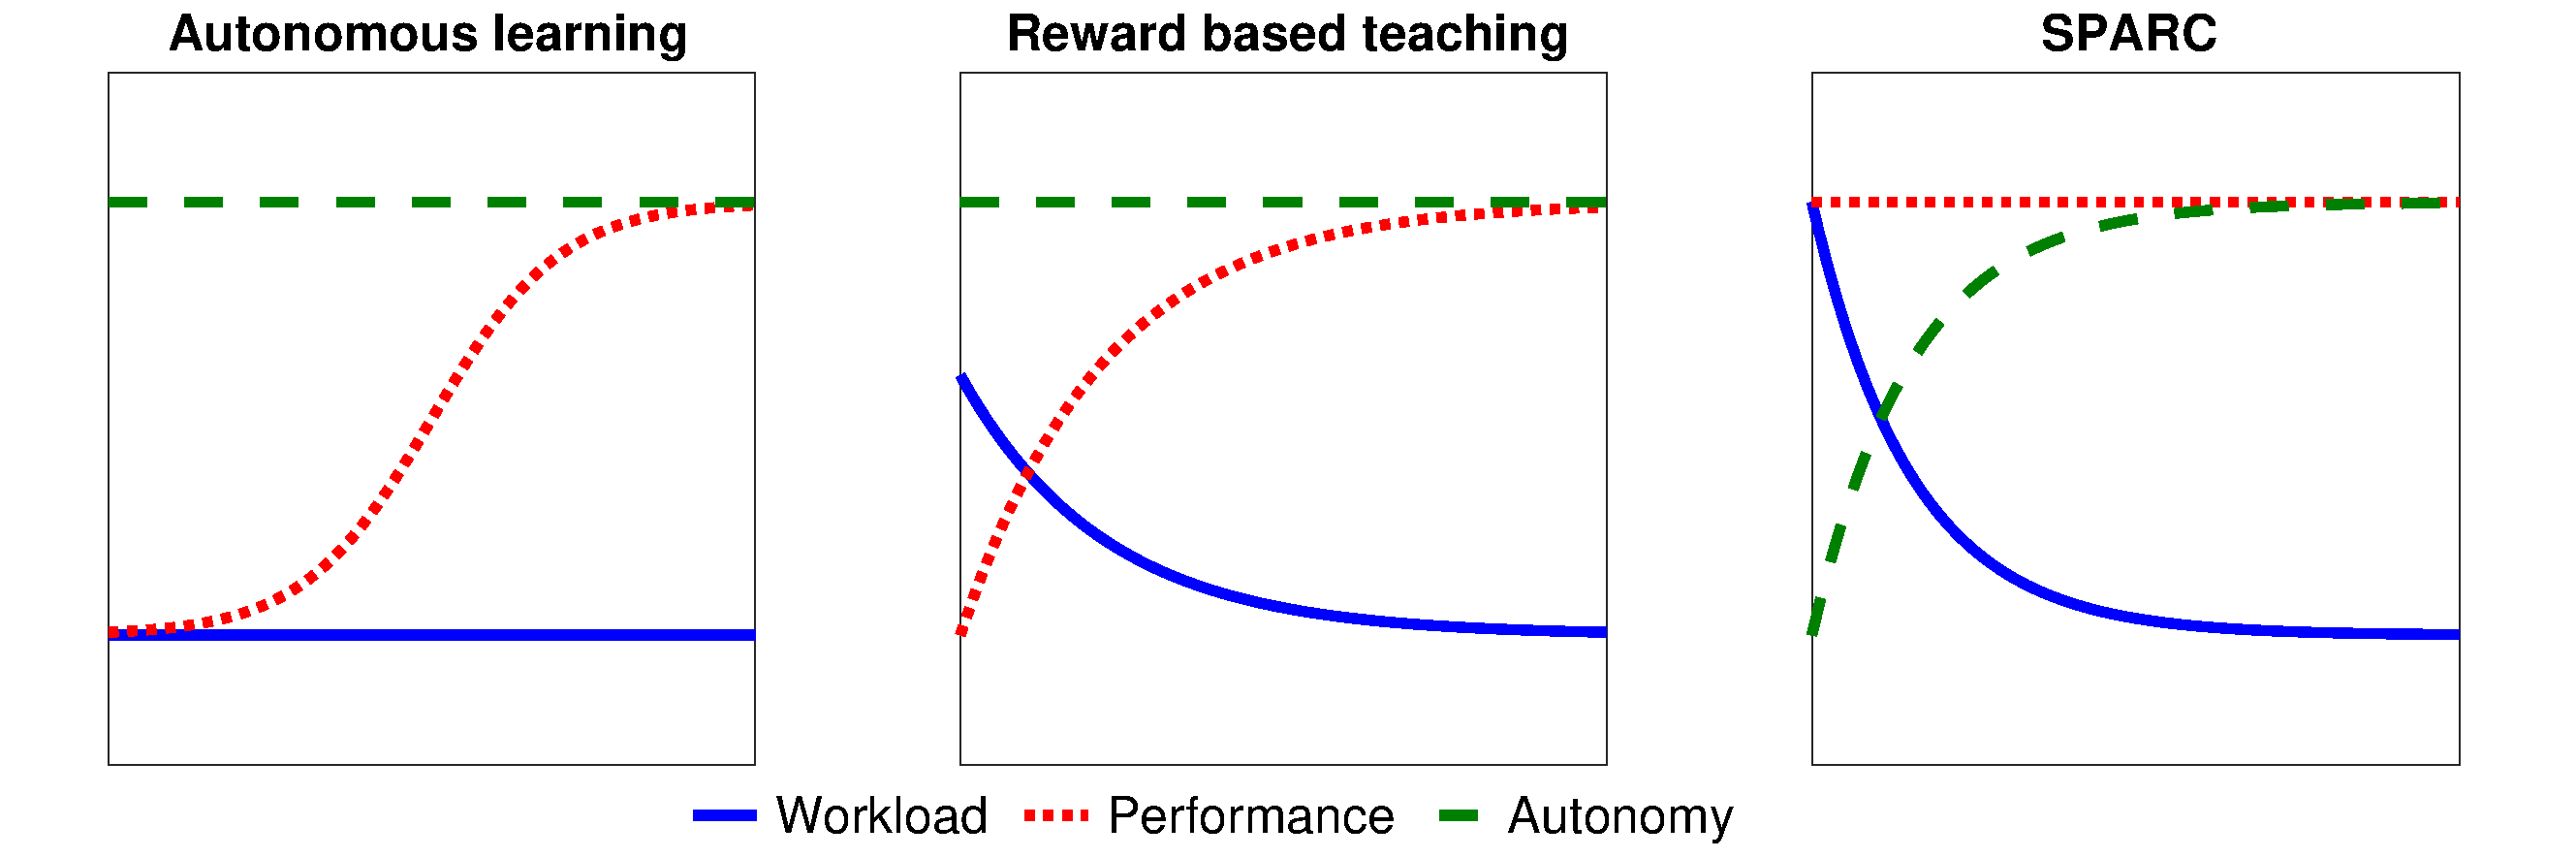
\includegraphics[width=0.9\linewidth]{./fig/motivation.pdf}
    \caption{Idealised expectation for performance, autonomy and human workload for a
    an autonomous learner, an approach using human rewards and SPARC.}
    \label{fig:comparison}
\end{figure}

%SPARC has been designed with the idea of teaching a robot to interact with humans,
%it is specially usefull when the frequency of action selection is low (less than
%1Hz) so action can be evaluated by a human before being executed, when the agent
%has to learn with a limited number of datapoints and when
%undesired actions executed by an agent can have a high cost and are to be
%avoided. 

In \cite{senft2017supervised}, we presented a way to combine SPARC and RL, by
assigning a positive reward to every action executed by the robot as it would
have been explicitely or implicitely approved by the supervisor. However this method
was not making use of any kind of generalisation, directly mapping a
single (state,action) pair to a reward, and as such is not applicable to
environments with a continuous or high dimensional space or undeterministic
transition from one state to another.

\section{Partial-State Supervised Reinforcement Learning}
\begin{comment}
Humans evolve in a highly complex environment with a nearly infinite number of
dimensions originating from different modality through our senses. But, despite
this complexity, we can select actions according to important features of the
state, regardless of other parts of it.

Taking inspiration from this observation, we argue that focusing on partial states, rather
than full states can both increase the speed of learning for an agent and
provide some of the generalisation required to interact in complex environment.
Guidance from a human can highlight important features in the state space and
associate them to actions. This shifts the state action pair paradigm to a
partial-state action pair, and in the case of RL, the tuple: partial-state,
action and reward. 
\end{comment}

To make RL applicable in high dimensional or continuous states, the algorithm
requires a way to generalise knowledge to unseen states. 
A classical approach is to use a first layer of neural
network or to use deep reinforcement learning which relies on deep neural
networks to learn a mapping state action Qvalue for example. 
These approaches, neural network based, relies on having a large number of
datapoints to converge toward a good function approximator. However, as
discussed previously, in many application, these amounts of data are not
possible to be obtained and methods to generalise quickly are more desirable.

%In \cite{sutton1996generalisation}, Sutton proposed to use sparse coarse
%coding
%dividing the state in slices and tiles as a way to generalise quickly for
%continuous spaces in RL. 

In this paper we propose to use a human to highlight the relevant features of
the environment to reduce the state dimension of the points stored in memory.
We introduce the concept of partial-state, a sliced version of the state defined
only on a subset of the dimensions of the state. This shifts the (state,action)
pair paradigm to (partial-state,action)  
and in the case of RL, the tuple (state, action, reward) to (partial-state,
action, reward).

\begin{comment}
%===============================================================================
\section{Methodology}

Similarly to a SPARC setup, the supervisor can select actions, or when presented
with an action about to be executed by the robot either cancel it or let
it be executed.

In addition to these actions, the supervisor can use the GUI to select features
of the environment that can be sent to the algorithm to reduce the state associated
to this action to a partial-state. Similarly, the algorithm can indicate which
parts of the states have been used for the selection to the supervisor who can
correct them while the action is being executed.

%Example?
\end{comment}

\subsection{Learning algorithm}

An expert supervises the agent actions, and can assign rewards to actions and
highlight the part of the states which are relevant to assigning this reward to
this partial-state.

As the supervisor can estimate the future impacts of an action, the problem of
credit assignment for delayed rewards can be ignored  and allows us to consider
only a myopic approach. 

For this paper, we will reuse the formalism of rewardless Markov Decision 
Process to identify the different elements of our system. The agent has access
to a set of actions $\mathcal{A}$, a state $\mathcal{S} \in [0,1]^{n}$. We
also define the partial-states $\mathcal{s'} \in [0,1]^{n'}$ with $n' \leq n$ as a
slice of $\mathcal{S}$, a subset of $\mathcal{S}$ where some dimensions have
been removed. 
%With each dimension of S representing features in the environment.

At the instant $t$, the agent has access the state $s$, an action $a$, evaluated
with a reward $r$ associated to the partial-state $s'$. For example, a state $s$ could be
defined in 4 dimensions such as ${s=[1,0.2,0,0.5]}$, and $s'$ in two dimensions with
${s'=[-,0.2,0,-]}$ with symbol '$-$' reprensenting the dimensions removed. The
action $a$ has been evaluated $r$ in the partial-state $s'$. 

To each action
$a \in \mathcal{A}$ we can associate a set $\mathcal{C}_{a}$ of pairs $(s',r)$
representing the rating done by the supervisor to action $a$ with feature
highlighted for $s'$. When adding a new pairt $(s',r)$, we can discard all the
previous pairs with an identical $s'$ to represent the evolution of the policy
evaluation by the supervisor.

\begin{algorithm}
    \DontPrintSemicolon
    \SetKwInOut{Input}{inputs}\SetKwInOut{Output}{output}
    \Input{Current state $s$, set of  $(a,s',r)$}
    \Output{selected action $\pi(s)$}
    \ForEach{$a \in \mathcal{A}$}{
        \ForEach{$(s'-r) \in \mathcal{C}_{a}$}{
            compute similarity $\Delta$ between $s$ and $s'$:
            $\Delta(s')=1-\frac{\sum_{i}^{n'}(s'(i)-s(i))^{2}}{n'}$
        }
        compute expected reward $\hat{r}(a)$:
        $\hat{r}(a) = max(\Delta) \cdot r(arg\, max_{s'} \Delta(s'))$\\
        with $r(\Delta(s'))$ reward of $(s'-r)$ pair
    }
    $\pi(s) = arg\, max_{a} \hat{r}(a)$

    \caption{Algorithm for selecting an action based on previous
    partial-state action rewards tuples and current state}
    \label{algo}
\end{algorithm}


When facing a new state $s$ where an action has to be
selected, the agent can select an action following Algorithm~\ref{algo}. For
each action $a \in \mathcal{A}$, we take the pair $(s',r)$ with the closest $s'$
to the current state (as defined by normalised distance over the dimensions
where $s'$ is defined). That way, each action $a$ can be associated to an
expected reward defined by the product between the similarity of the closest
partial-state known for $a$ and the reward obtained in that partial-state.
Finally, the action with the highest expected reward can be selected.

When selecting an action with following Algorithm~\ref{algo}, the agent can also use
the dimensions of the similar state $s'$ used for the selection to indicate the
supervisor which parts of the state have been used for the action selection.

\subsection{Combination with SPARC}

SPARC has been showed to be compatible with RL in \cite{senft2017supervised},
and can also be easily combined with the approach presented in paper using
partial states. For example, when selecting an action for the robot to be
executed, the supervisor can also select which features in the environment
should be selected in the partial state, and this associate the reward +1
to this action in this partial state. Similarly when an action is
proposed
to the supervisor the dimensions features represented by the dimensions of the
closest partial state can be explosed to the supervisor as a way to explain why
this action has been selected. Facing this, the supervisor can not react,
letting the action being executed and associating a reward of +1 to the partial
state and the action proposed, the supervisor could also change the partial
state to correct the features related to this action or cancel it, preventing the
execution and associating a reward of -1.

\section{Example of application}

An example of application yet to be tested is robot for teaching to children.
A robot can play an educative game with children to teach them notions about
diverse topics according to the needs of the teacher. For this example, a child
and a robot are playing a game about food web, teaching wich animals eat which
ones on a Sandtray~\cite{baxter2012touchscreen} as shown in
Figure~\ref{fig:game}. In addition to the child and
the robot, an adult supervises the robot using a tablet with a Graphical User
Interface (GUI) (Figure~\ref{fig:gui}) to teach the robot how to interact with the child.
\begin{figure}
        \centering
  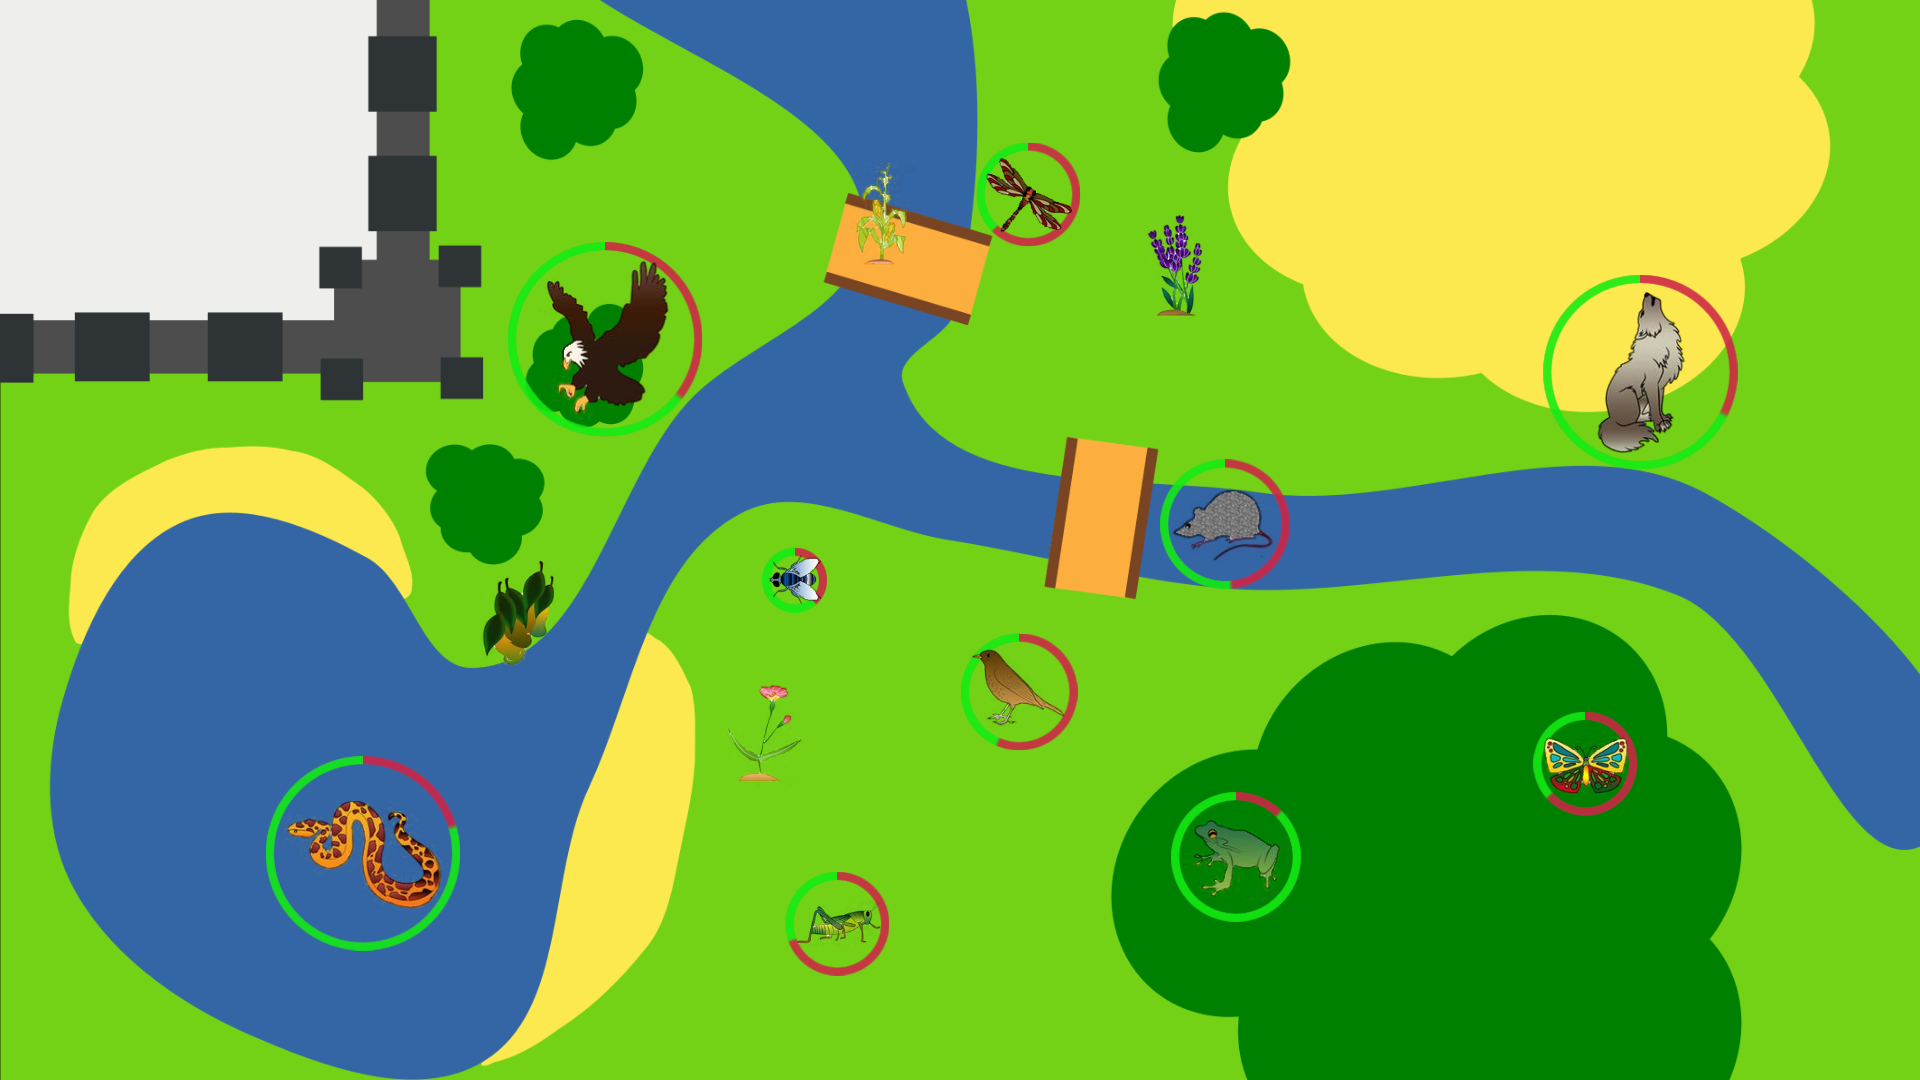
\includegraphics[width=80mm]{./fig/game.png} 
    \caption{Game displayed on the Sandtray the child is playing with the robot.}
        \label{fig:game}
\end{figure}

As shown in Figures \ref{fig:game} and \ref{fig:gui}, the GUI is an augmented
version of the game itself, which can be use to make the robot move items on the
game by dragging them on the GUI or which can display actions proposed by the
robot with a cancel button to refuse an action. For example in
Figure~\ref{fig:gui} the robot proposes to move the eagle to the rat, and
highlight (as shown by blue circles) the eagle and the rat. This indicate that
features relevant to the eagle and the rat have been used to select this action.
\begin{figure}
        \centering
    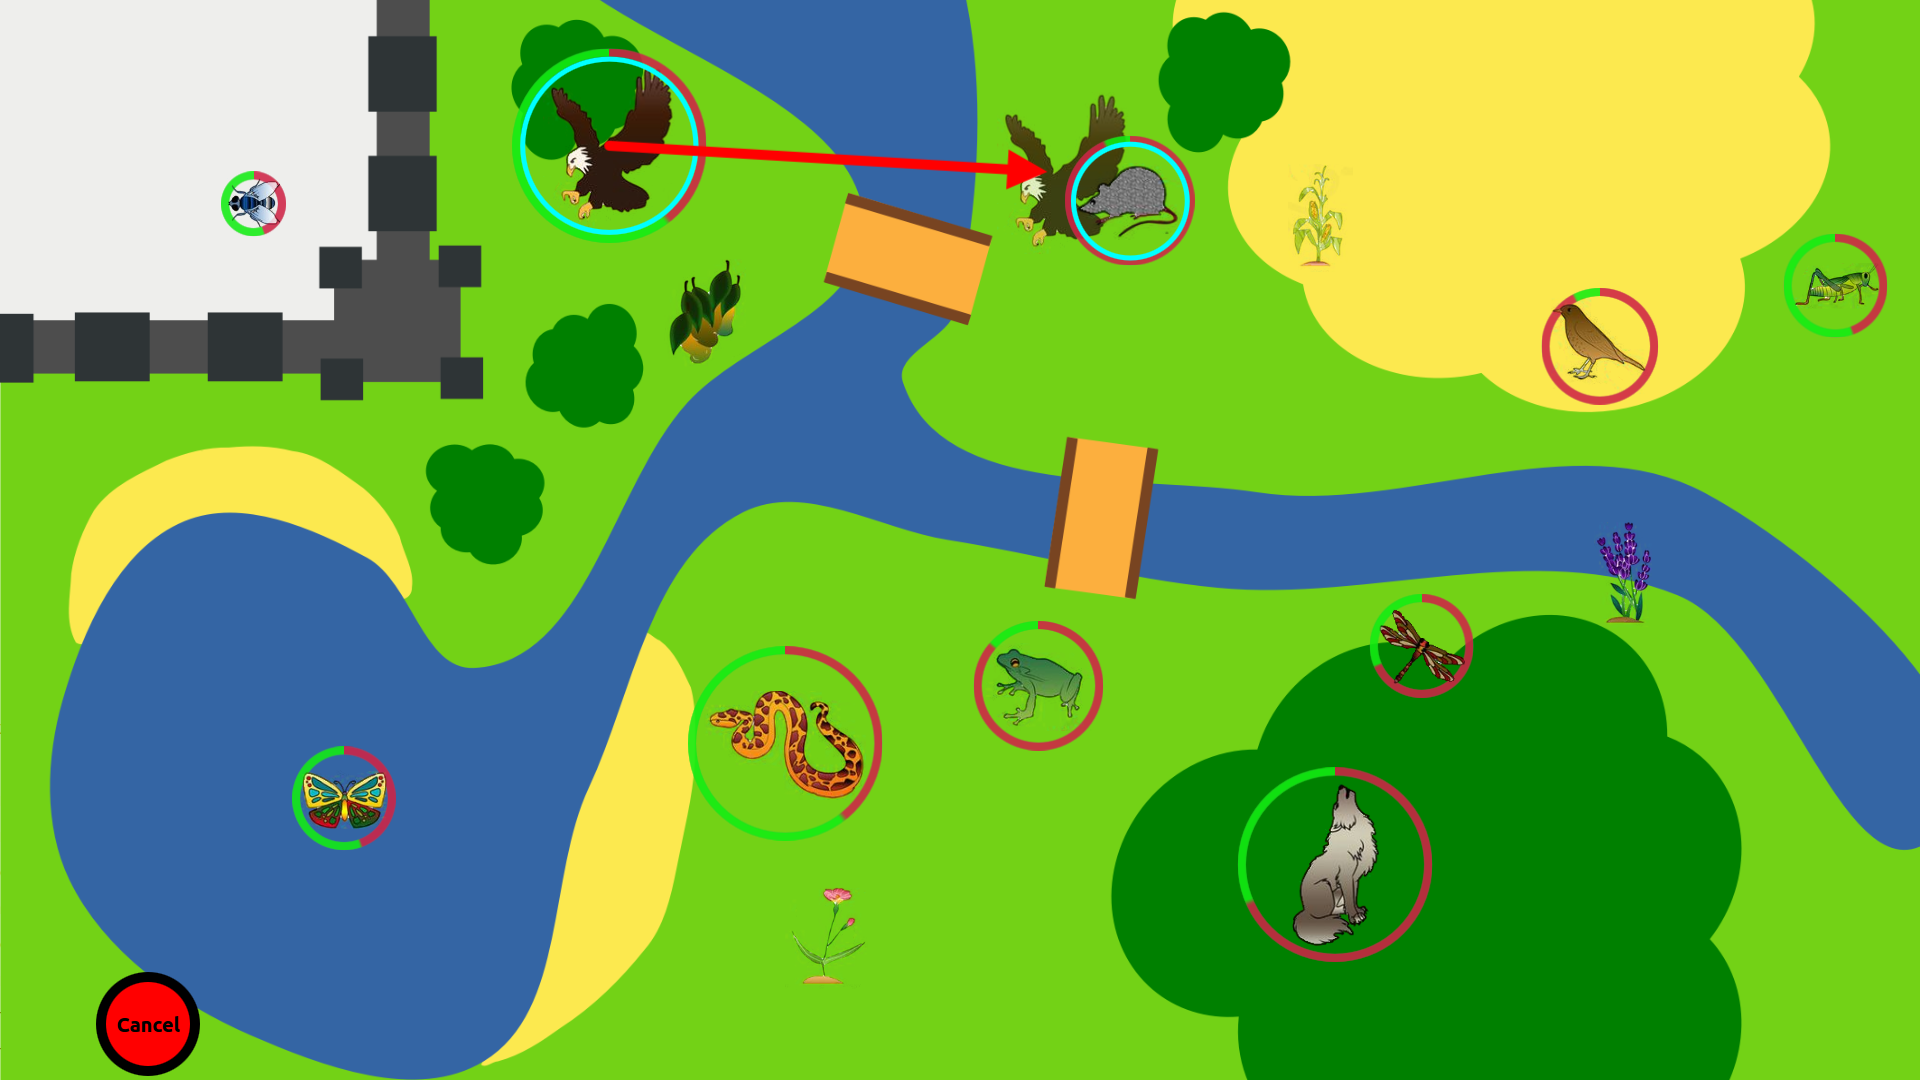
\includegraphics[width=80mm]{./fig/proposition.png}
    \caption{Interface for the supervisor with an action being proposed, moving
        eagle to rat with highlight of eagle and rat.}
        \label{fig:gui}
\end{figure}


In the current implementation, the state is defined by the distance between each
animals and their life. With these features selected, the partial state
transmitted to the user is the distance between the eagle, the eagle's life and
the rat's life. Similarly, when selected an action, the supervisor can also
select features in the state relevant to the selction.

Limitations of the approach reside in the difference of
representation of the state and action spaces between the supervisor and the
algorithm and limits in the communication. For example a user could try to move
an animal close to another one,
and depending of the represenation of the actions on the algorithm side, the
action might not be understood in the same way. Similarly, features used by the
supervisor to select actions might not be represented in the state used by the
algorithm. And lastly, in the case of implicit selection of features, a single
case of features representatin (for example highlighting two animals) might not
be perceived in the same way by observers.


%===============================================================================
\begin{comment}
\section{Challenges}

A large body of the
Interactive Machine Learning research is focused on simple inputs from the
humans, such as providing labels \cite{cakmak2012designing}, rewards
\cite{knox2009interactively} or kinesthetic demonstrations
\cite{billard2008robot}. However, as stated in \cite{amershi2014power}: "people
want to demonstrate how learners should behave" and "users may desire richer
control over machine-learning systems than simply labeling data". Human teachers
want to be more active and involved in the teaching process, to make their
student learning faster. 
And, as shown in \cite{senft2017supervised}, providing teacher with this control
can keep the agent in relevant states of the environment, speeding the learning
and reducing the risk to have the robot execute undesired actions.

In human social learning, both interactants have access to a similar set of
inputs: the senses available to a human body, and the teacher has additional
knowledge about the environment that can be communicated in an open ended way to
the learner. On the other in human-robot teaching, the way to sense the world
can be highly different between the two partners, and as of today, there is no
open ended way of communicating new concepts or explication as natural langage
processing is not yet solve. This creates two main challenges to make robot
learning for human use complex inputs: 
\begin{itemize}
    \item Having a mapping between the action state space of the human and the
            robot ensuring that feature used for action selection for one
            interactant are available to the other.
    \item Communicating these features from one participant to the other: allow
        the robot to make sense of the human's instructions and the human to
        understand the robot's intentions.
\end{itemize}
\end{comment}
\section{Future work}

The system presented in the previous section will be improved and
evaluated in the real world with children in the next months.

The current work could also be extended to allow the agent continue to improve its
behaviour even in the absence of supervisor, progressively exploring around the
learnt policy improving its behaviour beyond the demonstrations. This
could be done by allowing the supervisor to provide rewards during the learning
phase, and combine these rewards with the demonstrations to learn a reward
function in a fashion similar to Inverse Reinforcement Learning
\cite{abbeel2004apprenticeship}. These could also use partial states associated
to these rewards to ease the generalisation of the reward function with only a
low number of datapoints.
But without the supervisor, the assumption that only a
myopic action selection is sufficient would not hold anymore and the problem of
delayed rewards would have to be tackled.
%===============================================================================
%\section{Conclusion}
\label{sec:conclusion}
%==============================================================================
\section{Acknowledgments}
This work was supported by the EU FP7 DREAM project (grant no.  611391) and EU
H2020 Marie Sklodowska-Curie Actions project DoRoThy (grant 657227).  

\bibliographystyle{aaai} \bibliography{biblio}
\end{document}
